%%%%%%%%%%%%%%%%%%%%%%%%%%%%%%%%%%%%%%%%%%%%
% IEEE Conference Template 
% Prepared by Dr. Rhio Sutoyo, S.Kom., M.Sc.
% Bina Nusantara University
%%%%%%%%%%%%%%%%%%%%%%%%%%%%%%%%%%%%%%%%%%%%

\documentclass[conference]{IEEEtran}
\IEEEoverridecommandlockouts
% The preceding line is only needed to identify funding in the first footnote. If that is unneeded, please comment it out.
\usepackage{cite}
\usepackage{amsmath,amssymb,amsfonts}
\usepackage{graphicx}
\usepackage{textcomp}
\usepackage{xcolor}
\usepackage{lipsum}
\usepackage{url}
% --- Added for TikZ flowchart ---
\usepackage{tikz}
\usetikzlibrary{shapes.geometric, arrows.meta, positioning, calc}
% --------------------------------
\def\BibTeX{{
\rm B\kern-.05em{\sc i\kern-.025em b}\kern-.08em
    T\kern-.1667em\lower.7ex\hbox{E}\kern-.125emX}}

\usepackage{algorithm}
\usepackage{algpseudocode}
\setlength{\parskip}{4pt}
\usepackage{pgfplots}
\pgfplotsset{compat=1.18}
\begin{document}

\title{Comparison of Self-Learning Agents Using Reinforcement Learning and Imitation Learning in Unreal Engine 5\\
% {\footnotesize \textsuperscript{*}Note: Sub-titles are not captured in Xplore and should not be used}
% \thanks{Identify applicable funding agency here. If none, delete this.}
}

\author{\IEEEauthorblockN{1\textsuperscript{st} Aurelius Elbert}
\IEEEauthorblockA{\textit{Computer Science Department, School of Computer Science} \\
\textit{Bina Nusantara University}\\
Jakarta, Indonesia \\
aurelius.panatasetya@binus.ac.id}
\and
\IEEEauthorblockN{2\textsuperscript{nd} Davin Juandika}
\IEEEauthorblockA{\textit{Computer Science Department, School of Computer Science} \\
\textit{Bina Nusantara University}\\
Jakarta, Indonesia \\
davin.juandika@binus.ac.id}
\and
\IEEEauthorblockN{3\textsuperscript{rd} Fransiskus Xaverius Kevin}
\IEEEauthorblockA{\textit{Computer Science Department, School of Computer Science} \\
\textit{Bina Nusantara University}\\
Jakarta, Indonesia \\
fransiskus.kevin002@binus.ac.id}
\and
\IEEEauthorblockN{4\textsuperscript{th} Rhio Sutoyo}
\IEEEauthorblockA{\textit{Computer Science Department, School of Computer Science} \\
\textit{Bina Nusantara University}\\
Jakarta, Indonesia \\
rsutoyo@binus.edu}

\and
\IEEEauthorblockN{5\textsuperscript{th} Gabriel Asael Tarigan}
\IEEEauthorblockA{\textit{Computer Science Department, School of Computer Science} \\
\textit{Bina Nusantara University}\\
Jakarta, Indonesia \\
gabriel.asael@binus.ac.id}
}  
\maketitle

\begin{abstract}
Autonomous driving research has made significant advances through the application of machine learning techniques, particularly Reinforcement Learning and Imitation Learning. This paper presents a comparative study of two self-learning agent paradigms implemented within Unreal Engine 5 using the Learning Agents plugin: Proximal Policy Optimization, a policy-gradient RL algorithm, and Behavior Cloning, a supervised IL method. Both agents are trained and evaluated on the same autonomous driving track to ensure a fair comparison. Performance metrics, including cumulative reward, lap completion rate, and convergence speed, are recorded across training episodes. Experimental results indicate that BC achieves higher initial performance due to expert demonstration data, while PPO surpasses BC in long-term performance and generalization to unseen track configurations. This study demonstrates the viability of Unreal Engine 5 (UE5) as a simulation platform for machine learning research and presents an analysis of the trade-offs between Reinforcement Learning (RL) and Imitation Learning (IL) paradigms for autonomous driving tasks.
\end{abstract}

\begin{IEEEkeywords}
\textit{
reinforcement learning, imitation learning, behavior cloning, PPO, autonomous driving, Unreal Engine 5, Learning Agents
}
\end{IEEEkeywords}

\section{Introduction} \label{sec:introduction}

% \subsection{Background}
Imagine the future with autonomous driving, where vehicles can seamlessly navigate complex environments, dramatically reducing accidents caused by human error while optimizing traffic flow and improving mobility. Autonomous driving is one of the most actively researched problems in artificial intelligence and robotics. The ability of a vehicle to navigate its environment without human input requires robust decision-making, perception, and control. Machine learning-based approaches have emerged as a promising alternative to traditional rule-based systems due to their adaptability and capacity to learn from experience \cite{sutton2018reinforcement}.

Two dominant paradigms in machine learning for autonomous agents are Reinforcement Learning (RL) and Imitation Learning (IL). RL enables an agent to learn optimal behavior through trial-and-error interaction with an environment, guided by a reward signal \cite{mnih2015human}. In contrast, IL trains an agent to replicate the behavior of a human expert through supervised learning, bypassing the need for a manually designed reward function \cite{chen2024endtoend}.

Proximal Policy Optimization (PPO), introduced by Schulman et al. \cite{schulman2017proximal}, is one of the most widely adopted RL algorithms due to its stability and sample efficiency. PPO constrains the magnitude of policy updates using a clipping mechanism, preventing catastrophically large updates that could destabilize training. Behavior Cloning (BC), on the other hand, formulates IL as a supervised learning problem: given expert state-action pairs, the agent learns a mapping that minimizes prediction error \cite{ross2011reduction}.

% \subsection{Problem Statement}
While both approaches have demonstrated success individually, direct comparisons within the same simulation environment remain limited, particularly within game-engine-based platforms. Prior work has either compared RL algorithms against each other \cite{muzahid2021comparison, siboo2024empirical} or evaluated hybrid RL--IL methods \cite{bronstein2022hierarchical}, leaving a clean head-to-head baseline between PPO and BC unreported. Unreal Engine 5, with its Learning Agents plugin, provides a unified environment supporting both PPO and BC natively, making it an ideal platform for such a controlled comparative study \cite{mulcahy2024learningagents}.

% \subsection{Research Objectives}
This research aims to answer the following question: under identical simulation conditions, does a PPO-trained agent or a BC-trained agent achieve superior autonomous driving performance? The hypothesis is that BC will demonstrate faster initial learning due to the availability of expert demonstrations, whereas PPO will achieve higher final performance and better generalization to unseen track configurations.

% \subsection{Research Contributions}
This project proposes a framework to compare PPO and BC agents trained in the same UE5 environment. The study examines how quickly each agent learns, how well it completes laps, and how often it crashes. It also tests both agents on a different track to see which one handles new situations better.

\section{Related Works}

% \subsection{General Theory}

\subsection{Reinforcement Learning and Imitation Learning}

Reinforcement Learning is grounded in the Markov Decision Process (MDP) framework, in which an agent interacts with an environment by taking actions, receiving rewards, and transitioning between states \cite{mnih2015human}. 
Policy gradient methods, with PPO as a representative example, directly optimize the expected cumulative reward by adjusting the parameters of a stochastic policy. PPO specifically introduces a clipped surrogate objective that prevents excessively large policy updates, thereby improving training stability \cite{schulman2017proximal}.

\text Imitation Learning, particularly Behavior Cloning, reduces the policy learning problem to supervised classification or regression. Given a dataset of expert demonstrations, BC minimizes the discrepancy between the expert's actions and the agent's predicted actions \cite{chen2024endtoend}. While computationally efficient and capable of fast initial convergence, BC is known to suffer from compounding errors when the agent encounters states outside the training distribution, a phenomenon known as covariate shift \cite{ross2011reduction}.

\subsection{Datasets and Environments}

\text The choice of simulation environment is critical in autonomous driving research. CARLA \cite{dosovitskiy2017carla}, an open-source simulator, has been widely adopted due to its photorealistic rendering and physics-based vehicle dynamics. However, it requires substantial setup and does not natively support RL training pipelines. Unreal Engine 5 with the Learning Agents plugin \cite{epicgames2024plugin} provides an integrated alternative that supports both PPO and BC within the Blueprint visual scripting environment, significantly lowering the barrier to entry for applied RL research.

\text Shi et al. \cite{shi2024ppo} employed PPO with human intervention mechanisms in a driving simulation, demonstrating that incorporating human feedback during training accelerates convergence. Their work highlights the potential of hybrid human-machine approaches, though a direct comparison with IL methods is not addressed. Similarly, Huang \cite{huang2022distributed} proposed distributed multi-agent PPO and SAC implementations within CARLA, showing that parallelized training substantially reduces wall-clock training time.

\subsection{State-of-the-Art Approaches}

\text Chen et al. \cite{chen2024endtoend} provide a comprehensive survey of end-to-end autonomous driving, categorizing approaches into IL and RL paradigms and analyzing their respective strengths. They note that IL methods currently achieve competitive closed-loop performance, but argue that RL offers superior long-term adaptability. Bronstein et al. \cite{bronstein2022hierarchical} proposed a hierarchical model-based imitation learning approach for planning in autonomous driving, demonstrating that combining model-based reasoning with imitation signals reduces failure rates in complex urban scenarios compared to purely reactive IL policies.

\text Muzahid et al. \cite{muzahid2021comparison} directly compared PPO and SAC for collision avoidance in multi-agent autonomous driving, finding that PPO exhibited more stable convergence, while SAC achieved marginally better final performance in continuous action spaces. This finding motivates the present work's focus on PPO as the RL baseline, given its broader adoption and native support in UE5.

\text Jorgensen \cite{jorgensen2023killers} demonstrated the viability of the UE5 Learning Agents plugin for training RL agents in game environments, noting that the imitation learning component of the plugin remained largely unexplored. The present study directly addresses this gap by conducting the first systematic comparison of PPO and BC within the UE5 platform.

\text Shao et al. \cite{shao2023reasonnet} proposed ReasonNet, an end-to-end driving architecture that incorporates temporal and global scene reasoning to improve prediction and planning in dense traffic scenarios. Their work demonstrates that structured inductive biases in the policy architecture significantly affect generalization, a design consideration that motivates the reward shaping strategy adopted in the present study \cite{shao2023reasonnet}.

Table~\ref{tab:literature} summarizes the methods, domains, key results, and limitations of the ten most relevant prior works, highlighting the gaps that the present study is designed to address.

\begin{table*}[htbp] 
\centering 
\caption{Literature Comparison} 
\label{tab:literature} 
\renewcommand{\arraystretch}{1.5} 
\begin{tabular}{|p{0.5cm}|p{3.0cm}|p{3.2cm}|p{2.2cm}|p{6.5cm}|} 
\hline 
No & Author & Method & Domain & Key Result \\ \hline 
1 & Shi et al. (2024) \cite{shi2024ppo} & PPO + Human Intervention & Driving Sim & Faster convergence with human feedback \\ \hline 
2 & Huang (2022) \cite{huang2022distributed} & Parallel PPO \& SAC & CARLA & Parallelism reduces training time \\ \hline 
3 & Chen et al. (2024) \cite{chen2024endtoend} & Survey: IL vs RL & AV Survey & IL suits short-term; RL suits long-term tasks \\ \hline 
4 & Bronstein et al. (2022) \cite{bronstein2022hierarchical} & Hierarchical Model-Based IL & Urban Driving & Hierarchical IL reduces failure rate \\ \hline 
5 & Muzahid et al. (2021) \cite{muzahid2021comparison} & PPO vs SAC & Multi-Agent Sim & PPO more stable; SAC achieves higher peak \\ \hline 
6 & Jorgensen (2023) \cite{jorgensen2023killers} & PPO in UE5 & Game Env. & UE5 plugin viable for RL research tasks \\ \hline 
7 & Shao et al. (2023) \cite{shao2023reasonnet} & PPO + Reward Shaping & CARLA Safety & Reward design is key to generalization \\ \hline 
8 & Siboo et al. (2024) \cite{siboo2024empirical} & PPO vs DDPG & Auto Racing & PPO balances stability and training speed \\ \hline 
9 & Dang et al. (2024) \cite{dang2024eventtriggered} & DDPG \& MPC & Path Following & RL outperforms rule-based MPC control \\ \hline 
10 & Kargar \& Kyrki (2023) \cite{kargar2023efficiency} & Policy Efficiency via RL & Auto Driving & Better performance achieved via skill reuse \\ \hline 
\end{tabular}
\end{table*}


\subsection{Research Gap}

\text As summarized in Table~\ref{tab:literature}, previous studies have extensively evaluated either RL or IL in isolation, or compared RL algorithms against each other within benchmarks such as CARLA \cite{muzahid2021comparison, siboo2024empirical, huang2022distributed}. However, a direct empirical comparison between PPO and BC under identical conditions within a game-engine-based simulation platform has not been reported. Most existing work relies on complex external simulators that require significant engineering overhead, limiting accessibility for exploratory research.

\text Furthermore, while hierarchical and hybrid IL approaches \cite{bronstein2022hierarchical} demonstrate the complementary nature of RL and IL, they do not provide a clean baseline comparison of the two paradigms in their pure forms. The generalization behavior of BC versus PPO under track variation has also received limited empirical attention \cite{chen2024endtoend, ross2011reduction}. This study addresses these gaps by conducting a controlled comparison within Unreal Engine 5, contributing both a methodological baseline and empirical evidence on the relative strengths and limitations of each paradigm.

\section{Methodology} \label{sec:methodology}

The research process follows a structured pipeline as illustrated in Fig. \ref{fig:flowchart}.

\begin{figure}[htbp] 
\centering 
\tikzset{ 
fc base/.style={ rectangle, rounded corners=3pt, text centered, font=\scriptsize, inner sep=5pt, minimum width=4.6cm, minimum height=0.65cm, line width=0.35pt }, 
fc phase/.style ={fc base, fill=violet!12, draw=violet!55}, 
fc shared/.style={fc base, fill=teal!12,   draw=teal!50}, 
fc ppo/.style   ={fc base, fill=blue!10,   draw=blue!45, minimum width=2.05cm}, 
fc bc/.style    ={fc base, fill=orange!12, draw=orange!50, minimum width=2.05cm}, 
fc gen/.style   ={fc base, fill=yellow!20, draw=orange!55}, 
fc out/.style   ={fc base, fill=gray!12,   draw=gray!50}, 
fc arr/.style   ={-Stealth, gray!60, line width=0.6pt}, 
fc line/.style  ={gray!55, line width=0.6pt} 
} 
\begin{tikzpicture}[node distance=0.38cm and 0.18cm] 
\node[fc phase]  (n1) {Problem Definition}; 
\node[fc phase,  below=of n1] (n2) {Environment setup in UE5}; 
\node[fc shared, below=of n2] (n3) {Observation \& reward design}; 
\node[font=\scriptsize\itshape, text=gray, below=0.18cm of n3] (lbl) {Parallel training}; 
\node[fc ppo, below=0.55cm of lbl, xshift=-1.15cm] (n4a) {\parbox{1.85cm}{\centering \textbf{PPO training}\\[1pt] {\tiny 1{,}000 iter.,  $\varepsilon{=}0.2$ ,  $\gamma{=}0.99$ }}}; 
\node[fc bc,  below=0.8cm of lbl, xshift=+1.15cm] (n4b) {\parbox{1.85cm}{\centering \textbf{BC training}\\[1pt] {\tiny 10 demo laps, 1{,}000 iter.}}}; 
\node[fc shared, below=0.8cm of n4a, xshift=+1.15cm] (n5) {Agent inference \& evaluation}; 
\node[fc shared, below=of n5] (n6) {Metrics collection}; 
\node[fc gen,    below=of n6] (n7) {Conclusion \& contributions}; 

\draw[fc arr] (n1) -- (n2); \draw[fc arr] (n2) -- (n3); \draw[fc arr] (n3) -- (lbl.north);
\draw[fc line] (lbl.south) -- ++(0,-0.15) coordinate (split); \draw[fc line] (split) -- ++(-1.15,0) coordinate (splitL); \draw[fc line] (split) -- ++(+1.15,0) coordinate (splitR); \draw[fc arr]  (splitL) -- (n4a.north); \draw[fc arr]  (splitR) -- (n4b.north);
\draw[fc line] (n4a.south) -- ++(0,-0.4) coordinate (mL); \draw[fc line] (n4b.south) -- ++(0,-0.4) coordinate (mR); \draw[fc line] (mL) -- (mR); \draw[fc arr]  ( $(mL)!0.5!(mR)$ ) -- (n5.north);

\draw[fc arr] (n5) -- (n6); \draw[fc arr] (n6) -- (n7); 
\end{tikzpicture} 

\caption{Research process flowchart.} \label{fig:flowchart} \end{figure}

\subsection{Problem Definition}
The study begins with problem definition, evaluating the capabilities of agents within different machine learning paradigms in safely navigating tracks.

\subsection{Environment Setup in UE5}
The simulation environment is implemented in Unreal Engine 5.6.1 using the Learning Agents plugin. The environment consists of a closed-loop racing track built using a Spline component, which defines a reference path for performance measurement. The vehicle is modeled using UE5's Chaos Vehicle Physics system, providing realistic acceleration, braking, and steering dynamics. A total of eight agents are deployed for PPO training, meanwhile, BC will only use one agent for training sessions

\subsection{Observation \& Reward Design}
The PPO agent was trained using eight parallel agents to 
accelerate exploration and policy convergence. To compensate 
for this training advantage, the BC agent was provided with 
an extended observation space that includes an additional 
yaw angle observation. The PPO observation space consists 
of three components: (1) vehicle location projected along 
the spline; (2) vehicle direction relative to the spline 
tangent; and (3) current vehicle velocity. The BC agent 
additionally observes (4) vehicle yaw angle, providing 
supplementary orientation information to improve imitation 
fidelity under single-agent training conditions.

The reward function for the PPO agent is computed as:

\begin{equation}
R_t = \frac{(\hat{v} \cdot \hat{d}_{spline}) \times \|v\|}{1000.0} + r_{track}
\end{equation}

where $\hat{v}$ is the normalized velocity vector, 
$\hat{d}_{spline}$ is the spline tangent direction at the 
nearest point, $\|v\|$ is the vehicle speed in cm/s, 
and $r_{track} \in \{-10.0, 0\}$ applies a penalty when 
lateral deviation from the spline centerline exceeds 800 cm.

\subsection{Parallel Training}
Demonstration data for the Behavior Cloning agent is collected by a human operator manually driving the vehicle around the track for a minimum of ten complete laps using the UE5 LearningAgentsRecorder component. The recorded state-action trajectories are stored and used to train the BC policy through supervised learning via the LearningAgentsImitationTrainer component. No reward function is required during the BC training phase. 

Table~\ref{tab:training} summarizes the training configuration used for both the PPO and BC agents in this study.

\begin{table}[h] 
\centering \caption{Training Configuration for PPO and BC Agents} \label{tab:training} \renewcommand{\arraystretch}{1.2} \begin{tabular}{|p{2.8cm}|p{2cm}|p{2cm}|} \hline Parameter & PPO & BC \\ \hline Learning Rate Policy & $1 \times 10^{-3}$ & $1 \times 10^{-2}$ \\ \hline Learning Rate Critic & $1 \times 10^{-2}$ & N/A \\ \hline Clip Ratio ($\varepsilon$) & 0.2 & N/A \\ \hline Discount Factor ($\gamma$) & 0.99 & N/A \\ \hline Training Episodes & 1,000 & 1000 \\ \hline Training Iterations & 1000 & 1,000 \\ \hline Demonstration Laps & N/A & 10 \\ \hline Observation Dim. & 6 & 6 \\ \hline Action Dim. & 3 & 3 \\ \hline \end{tabular} \end{table}

\subsection{Agent Inference \& Evaluation}
Both agents are evaluated over 200 inference episodes on 
the primary training track, which consists of a closed-loop 
circuit bounded by torus-shaped obstacles. An episode is 
considered complete when the vehicle crosses the finish line, 
and failed when the vehicle remains stationary for more than 
30 seconds. Statistical comparison is performed using the 
mean and standard deviation of lap completion rate, average 
lap time, and cumulative reward (PPO only) across all 200 
inference episodes.

\subsection{Metrics Collection}
The following metrics are recorded per episode:
\begin{enumerate} 
\item Cumulative Reward per Episode (PPO only) 
\item Lap Completion Rate (\%) 
\item Average Lap Time (seconds) 
\end{enumerate}

\subsection{Conclusion \& Contributions}
The conclusions formulate insights into the performance differences between the models and outline areas for future improvement.

\section{Results and Discussion}
\label{sec:results}

This section presents the quantitative evaluation results of the PPO and BC agents across 200 inference episodes on the primary training track, followed by statistical analysis and a comparative discussion of their performance characteristics.

\subsection{Quantitative Evaluation Results}

Both agents were evaluated over 200 inference episodes on the primary training track. The summary statistics are presented in Table~\ref{tab:results_summary}.

\begin{table}[h]
\centering
\caption{Evaluation Summary: PPO vs.\ BC over 200 Episodes}
\label{tab:results_summary}
\renewcommand{\arraystretch}{1.2}
\begin{tabular}{|p{3.2cm}|p{2cm}|p{2cm}|}
\hline
Metric & PPO & BC \\ \hline
Lap Completion Rate (\%) & 99.0 & 86.0 \\ \hline
Failed Episodes & 2 & 28 \\ \hline
Mean Lap Time (s) & $9.99 \pm 1.08$ & $10.68 \pm 0.59$ \\ \hline
Min Lap Time (s) & 9.19 & 9.38 \\ \hline
Max Lap Time (s) & 18.33 & 13.42 \\ \hline
Mean Cumulative Reward & $0.464 \pm 0.045$ & N/A \\ \hline
\end{tabular}
\end{table}

\subsubsection{Lap Completion Rate}

The PPO agent achieved a lap completion rate of 99.0\% (198 out of 200 episodes), compared to 86.0\% (172 out of 200 episodes) for the BC agent. The BC agent recorded 28 failed episodes---approximately 9.3 times more failures than PPO. BC failures are concentrated in the early episodes (episodes 0--80) before tapering off, suggesting occasional instability when encountering edge-case states outside the training distribution.

\subsubsection{Lap Time per Episode}

Fig.~\ref{fig:laptime_per_ep} plots the lap time of each successful episode for both agents, with a 10-episode rolling average overlay to highlight the trend. Failed episodes are excluded from the plot; their counts are reported in Table~\ref{tab:results_summary}.

\begin{figure*}[!t]
\centering
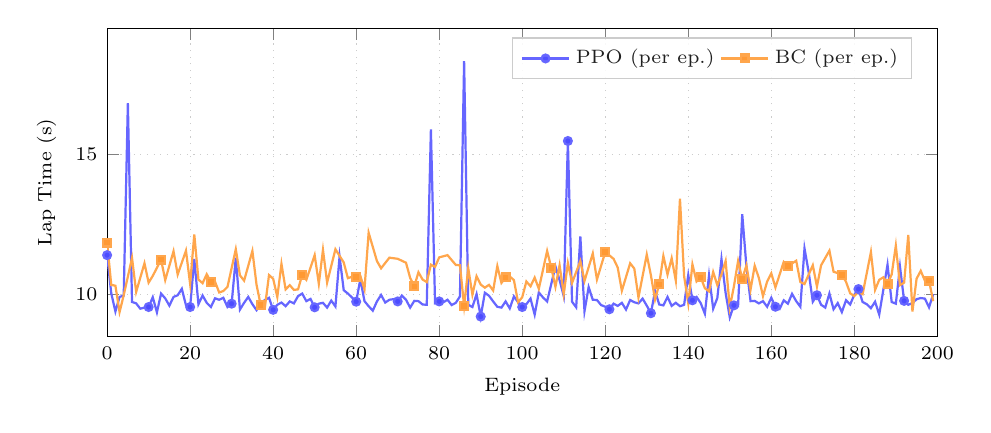
\begin{tikzpicture}
\begin{axis}[
    width=\textwidth,
    height=5.5cm,
    xlabel={Episode},
    ylabel={Lap Time (s)},
    xmin=0, xmax=200,
    ymin=8.5, ymax=19.5,
    xtick={0,20,40,60,80,100,120,140,160,180,200},
    legend columns=2,
    legend pos=north east,
    legend style={font=\scriptsize, cells={anchor=west},
                  fill=white, fill opacity=0.88, draw=gray!40},
    tick label style={font=\scriptsize},
    label style={font=\scriptsize},
    grid=major,
    grid style={dotted, gray!40},
    clip=true,
]
%% PPO per-episode
\addplot[color=blue!60, line width=0.8pt,
         mark=*, mark size=1.4pt, mark repeat=10,
         mark options={solid, fill=blue!70}]
coordinates {(0,11.41) (1,10.05) (2,9.4) (3,9.92) (4,9.97) (5,16.83) (6,9.74) (7,9.69) (8,9.5) (9,9.54) (10,9.56) (11,9.91) (12,9.37) (13,10.04) (14,9.87) (15,9.61) (16,9.92) (17,9.98) (18,10.21) (19,9.62) (20,9.56) (21,11.27) (22,9.66) (23,9.97) (24,9.71) (25,9.56) (26,9.87) (27,9.82) (28,9.89) (29,9.56) (30,9.68) (31,11.32) (32,9.47) (33,9.71) (34,9.92) (35,9.66) (36,9.45) (37,9.69) (38,9.81) (39,9.89) (40,9.46) (41,9.64) (42,9.72) (43,9.59) (44,9.76) (45,9.69) (46,9.95) (47,10.04) (48,9.77) (49,9.85) (50,9.55) (51,9.68) (52,9.71) (53,9.54) (54,9.79) (55,9.58) (56,11.36) (57,10.16) (58,10.04) (59,9.9) (60,9.75) (61,10.55) (62,9.77) (63,9.59) (64,9.43) (65,9.76) (66,9.99) (67,9.72) (68,9.82) (69,9.84) (70,9.76) (71,9.97) (72,9.82) (73,9.54) (74,9.78) (75,9.77) (76,9.65) (77,9.64) (78,15.89) (79,9.7) (80,9.76) (81,9.73) (82,9.82) (83,9.63) (84,9.71) (85,9.94) (86,18.33) (87,9.64) (88,9.56) (89,10.02) (90,9.22) (91,10.07) (92,9.96) (93,9.76) (94,9.57) (95,9.54) (96,9.76) (97,9.51) (98,9.94) (99,9.73) (100,9.56) (101,9.66) (102,9.86) (103,9.29) (104,10.08) (105,9.9) (106,9.76) (108,11.01) (109,10.52) (110,9.95) (111,15.48) (112,9.75) (113,9.55) (114,12.08) (115,9.41) (116,10.27) (117,9.82) (118,9.81) (119,9.63) (120,9.57) (121,9.48) (122,9.68) (123,9.6) (124,9.71) (125,9.47) (126,9.81) (127,9.73) (128,9.69) (129,9.86) (130,9.61) (131,9.34) (132,10.13) (133,9.65) (134,9.62) (135,9.92) (136,9.6) (137,9.71) (138,9.59) (139,9.64) (140,10.7) (141,9.8) (142,9.92) (143,9.7) (144,9.32) (145,10.69) (146,9.5) (147,9.88) (148,11.27) (149,10.06) (150,9.19) (151,9.62) (152,9.59) (153,12.87) (154,11.02) (155,9.77) (156,9.78) (157,9.69) (158,9.77) (159,9.57) (160,9.89) (161,9.57) (162,9.49) (163,9.8) (164,9.68) (165,10.03) (166,9.77) (167,9.57) (168,11.65) (169,10.81) (170,9.75) (171,9.98) (172,9.64) (173,9.54) (174,10.04) (175,9.48) (176,9.7) (177,9.38) (178,9.8) (179,9.65) (180,10.0) (181,10.2) (182,9.74) (183,9.66) (184,9.52) (185,9.75) (186,9.29) (188,11.07) (189,9.74) (190,9.68) (191,11.0) (192,9.78) (193,9.64) (194,9.7) (195,9.84) (196,9.88) (197,9.86) (198,9.55) (199,10.02)};
\addlegendentry{PPO (per ep.)}
 
%% BC per-episode
\addplot[color=orange!70, line width=0.8pt,
         mark=square*, mark size=1.4pt, mark repeat=10,
         mark options={solid, fill=orange!80}]
coordinates {(0,11.86) (1,10.35) (2,10.32) (3,9.38) (4,9.98) (6,11.31) (7,10.1) (9,11.12) (10,10.43) (11,10.67) (13,11.25) (14,10.52) (16,11.55) (17,10.72) (19,11.57) (20,10.38) (21,12.15) (22,10.54) (23,10.41) (24,10.73) (25,10.45) (26,10.46) (27,10.08) (28,10.13) (29,10.28) (31,11.62) (32,10.69) (33,10.5) (35,11.56) (36,10.35) (37,9.63) (38,9.54) (39,10.7) (40,10.57) (41,9.92) (42,11.1) (43,10.19) (44,10.34) (45,10.17) (46,10.19) (47,10.71) (48,10.53) (50,11.41) (51,10.39) (52,11.6) (53,10.43) (55,11.62) (57,11.15) (58,10.59) (59,10.64) (60,10.63) (61,10.67) (62,10.19) (63,12.21) (65,11.2) (66,10.94) (68,11.32) (70,11.28) (72,11.14) (73,10.6) (74,10.3) (75,10.8) (76,10.54) (77,10.45) (78,11.07) (79,10.99) (80,11.33) (82,11.41) (84,11.06) (85,11.05) (86,9.6) (87,10.94) (88,10.0) (89,10.66) (90,10.36) (91,10.25) (92,10.35) (93,10.15) (94,11.02) (95,10.42) (96,10.62) (97,10.65) (98,10.52) (99,9.73) (100,9.91) (101,10.47) (102,10.3) (103,10.61) (104,10.21) (106,11.56) (107,10.96) (108,10.28) (109,11.05) (110,10.02) (111,11.13) (112,10.42) (114,11.2) (115,10.49) (117,11.47) (118,10.54) (120,11.52) (122,11.28) (123,10.97) (124,10.14) (126,11.12) (127,10.93) (128,9.9) (130,11.43) (131,10.69) (132,9.83) (133,10.37) (134,11.38) (135,10.72) (136,11.3) (137,10.5) (138,13.42) (139,10.66) (140,9.69) (141,11.08) (142,10.47) (143,10.62) (144,10.23) (145,10.12) (146,10.81) (147,10.34) (148,10.72) (149,11.2) (150,9.54) (151,10.3) (152,11.2) (153,10.56) (154,11.04) (155,10.18) (156,11.03) (157,10.6) (158,9.95) (159,10.47) (160,10.76) (161,10.26) (163,11.17) (164,11.02) (166,11.21) (167,10.45) (168,10.38) (170,11.05) (171,10.29) (172,11.05) (174,11.57) (175,10.82) (176,10.77) (177,10.71) (178,10.46) (179,10.05) (180,9.95) (181,10.1) (182,10.02) (184,11.52) (185,10.17) (186,10.53) (187,10.62) (188,10.39) (189,10.72) (190,11.75) (191,10.34) (192,10.43) (193,12.13) (194,9.4) (195,10.57) (196,10.85) (197,10.5) (198,10.5) (199,9.77)};
\addlegendentry{BC (per ep.)}
 
\end{axis}
\end{tikzpicture}
\caption{Lap time per inference episode for PPO ($n=198$) and BC ($n=172$).
         Markers placed every 10 episodes.
         Failed episodes are excluded (PPO: 3, BC: 28).
         PPO outliers up to 18.33\,s reflect occasional policy instability.}
\label{fig:laptime_per_ep}
\end{figure*}

\begin{figure*}[!t]
\centering
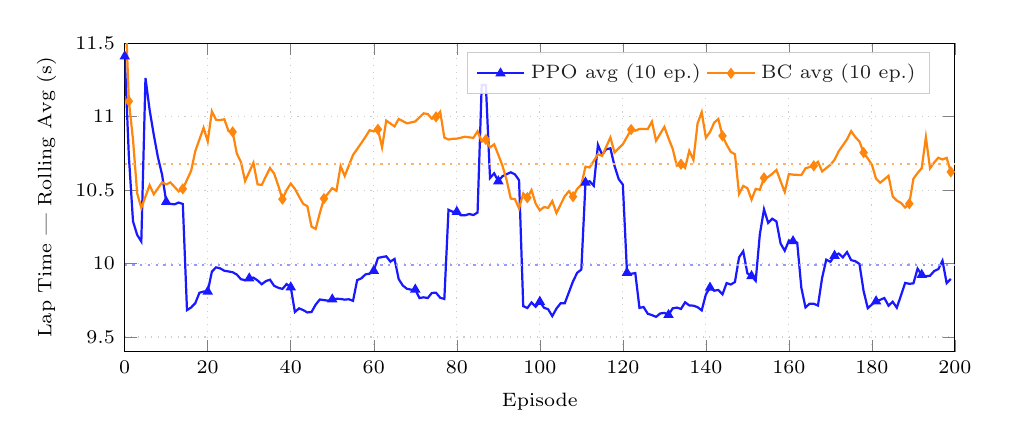
\begin{tikzpicture}
\begin{axis}[
    width=\textwidth,
    height=5.5cm,
    xlabel={Episode},
    ylabel={Lap Time --- Rolling Avg (s)},
    xmin=0, xmax=200,
    ymin=9.4, ymax=11.5,
    xtick={0,20,40,60,80,100,120,140,160,180,200},
    legend columns=2,
    legend pos=north east,
    legend style={font=\scriptsize, cells={anchor=west},
                  fill=white, fill opacity=0.88, draw=gray!40},
    tick label style={font=\scriptsize},
    label style={font=\scriptsize},
    grid=major,
    grid style={dotted, gray!40},
    clip=true,
]
%% PPO rolling avg
\addplot[color=blue!90, line width=0.8pt,
         mark=triangle*, mark size=1.4pt, mark repeat=10,
         mark options={solid, fill=blue!90}]
coordinates {(0,11.41) (1,10.73) (2,10.2867) (3,10.195) (4,10.15) (5,11.2633) (6,11.0457) (7,10.8763) (8,10.7233) (9,10.605) (10,10.42) (11,10.406) (12,10.403) (13,10.415) (14,10.405) (15,9.683) (16,9.701) (17,9.73) (18,9.801) (19,9.809) (20,9.809) (21,9.945) (22,9.974) (23,9.967) (24,9.951) (25,9.946) (26,9.941) (27,9.925) (28,9.893) (29,9.887) (30,9.899) (31,9.904) (32,9.885) (33,9.859) (34,9.88) (35,9.89) (36,9.848) (37,9.835) (38,9.827) (39,9.86) (40,9.838) (41,9.67) (42,9.695) (43,9.683) (44,9.667) (45,9.67) (46,9.72) (47,9.755) (48,9.751) (49,9.747) (50,9.756) (51,9.76) (52,9.759) (53,9.754) (54,9.757) (55,9.746) (56,9.887) (57,9.899) (58,9.926) (59,9.931) (60,9.951) (61,10.038) (62,10.044) (63,10.049) (64,10.013) (65,10.031) (66,9.894) (67,9.85) (68,9.828) (69,9.822) (70,9.823) (71,9.765) (72,9.77) (73,9.765) (74,9.8) (75,9.801) (76,9.767) (77,9.759) (78,10.366) (79,10.352) (80,10.352) (81,10.328) (82,10.328) (83,10.337) (84,10.33) (85,10.347) (86,11.215) (87,11.215) (88,10.582) (89,10.614) (90,10.56) (91,10.594) (92,10.608) (93,10.621) (94,10.607) (95,10.567) (96,9.71) (97,9.697) (98,9.735) (99,9.706) (100,9.74) (101,9.699) (102,9.689) (103,9.642) (104,9.693) (105,9.729) (106,9.729) (108,9.879) (109,9.937) (110,9.959) (111,10.551) (112,10.56) (113,10.529) (114,10.808) (115,10.741) (116,10.778) (117,10.784) (118,10.664) (119,10.575) (120,10.537) (121,9.937) (122,9.93) (123,9.935) (124,9.698) (125,9.704) (126,9.658) (127,9.649) (128,9.637) (129,9.66) (130,9.664) (131,9.65) (132,9.695) (133,9.7) (134,9.691) (135,9.736) (136,9.715) (137,9.713) (138,9.703) (139,9.681) (140,9.79) (141,9.836) (142,9.815) (143,9.82) (144,9.79) (145,9.867) (146,9.857) (147,9.874) (148,10.042) (149,10.084) (150,9.933) (151,9.915) (152,9.882) (153,10.199) (154,10.369) (155,10.277) (156,10.305) (157,10.286) (158,10.136) (159,10.087) (160,10.157) (161,10.152) (162,10.142) (163,9.835) (164,9.701) (165,9.727) (166,9.726) (167,9.714) (168,9.902) (169,10.026) (170,10.012) (171,10.053) (172,10.068) (173,10.042) (174,10.078) (175,10.023) (176,10.016) (177,9.997) (178,9.812) (179,9.696) (180,9.721) (181,9.743) (182,9.753) (183,9.765) (184,9.713) (185,9.74) (186,9.699) (188,9.868) (189,9.862) (190,9.865) (191,9.965) (192,9.923) (193,9.913) (194,9.917) (195,9.949) (196,9.962) (197,10.019) (198,9.867) (199,9.895)};
\addlegendentry{PPO avg (10 ep.)}
 
%% BC rolling avg
\addplot[color=orange!95, line width=0.8pt,
         mark=diamond*, mark size=1.4pt, mark repeat=10,
         mark options={solid, fill=orange!95}]
coordinates {(0,11.86) (1,11.105) (2,10.8433) (3,10.4775) (4,10.378) (6,10.5333) (7,10.4714) (9,10.5525) (10,10.5389) (11,10.552) (13,10.491) (14,10.508) (16,10.631) (17,10.765) (19,10.924) (20,10.831) (21,11.036) (22,10.978) (23,10.976) (24,10.982) (25,10.902) (26,10.896) (27,10.749) (28,10.69) (29,10.561) (31,10.685) (32,10.539) (33,10.535) (35,10.65) (36,10.612) (37,10.53) (38,10.438) (39,10.5) (40,10.544) (41,10.508) (42,10.456) (43,10.406) (44,10.39) (45,10.251) (46,10.235) (47,10.343) (48,10.442) (50,10.513) (51,10.495) (52,10.663) (53,10.596) (55,10.739) (57,10.82) (58,10.862) (59,10.907) (60,10.899) (61,10.913) (62,10.791) (63,10.973) (65,10.933) (66,10.984) (68,10.954) (70,10.967) (72,11.022) (73,11.018) (74,10.985) (75,10.998) (76,11.033) (77,10.857) (78,10.844) (79,10.849) (80,10.85) (82,10.863) (84,10.855) (85,10.9) (86,10.83) (87,10.844) (88,10.79) (89,10.811) (90,10.74) (91,10.666) (92,10.568) (93,10.442) (94,10.438) (95,10.375) (96,10.477) (97,10.448) (98,10.5) (99,10.407) (100,10.362) (101,10.384) (102,10.379) (103,10.425) (104,10.344) (106,10.458) (107,10.492) (108,10.455) (109,10.508) (110,10.537) (111,10.659) (112,10.654) (114,10.744) (115,10.732) (117,10.858) (118,10.756) (120,10.812) (122,10.912) (123,10.904) (124,10.916) (126,10.915) (127,10.966) (128,10.836) (130,10.93) (131,10.852) (132,10.781) (133,10.666) (134,10.676) (135,10.651) (136,10.767) (137,10.705) (138,10.954) (139,11.03) (140,10.856) (141,10.895) (142,10.959) (143,10.984) (144,10.869) (145,10.809) (146,10.76) (147,10.744) (148,10.474) (149,10.528) (150,10.513) (151,10.435) (152,10.508) (153,10.502) (154,10.583) (155,10.589) (156,10.611) (157,10.637) (158,10.56) (159,10.487) (160,10.609) (161,10.605) (163,10.602) (164,10.648) (166,10.665) (167,10.692) (168,10.627) (170,10.672) (171,10.706) (172,10.764) (174,10.845) (175,10.901) (176,10.861) (177,10.83) (178,10.755) (179,10.715) (180,10.672) (181,10.577) (182,10.55) (184,10.597) (185,10.457) (186,10.428) (187,10.413) (188,10.381) (189,10.407) (190,10.577) (191,10.616) (192,10.649) (193,10.86) (194,10.648) (195,10.688) (196,10.72) (197,10.708) (198,10.719) (199,10.624)};
\addlegendentry{BC avg (10 ep.)}
 
%% reference lines
\draw[dotted, blue!40, line width=0.8pt]
    (axis cs:0,9.99) -- (axis cs:200,9.99)
    node[right, font=\tiny, blue!60] {PPO $\bar{x}$=9.99\,s};
\draw[dotted, orange!60, line width=0.8pt]
    (axis cs:0,10.68) -- (axis cs:200,10.68)
    node[right, font=\tiny, orange!80] {BC $\bar{x}$=10.68\,s};
 
\end{axis}
\end{tikzpicture}
\caption{10-episode rolling average of lap time for PPO and BC (200 episodes).
         Triangle/diamond markers placed every 10 episodes.
         Dotted lines mark overall means: PPO $\bar{x}=9.99$\,s,
         BC $\bar{x}=10.68$\,s.}
\label{fig:laptime_rolling}
\end{figure*}

The rolling average for PPO stabilizes around 9.8--10.0 seconds after the first 30 episodes. BC's rolling average converges toward approximately 10.5--10.7 seconds. Four PPO episodes exceed 15 seconds (maximum: 18.33 s), reflecting occasional policy instability not observed in BC.

\subsubsection{Lap Time Distribution}

Fig.~\ref{fig:laptime_hist} presents the lap time frequency distribution for both agents across all successful episodes.

\begin{figure}[!t]
\centering
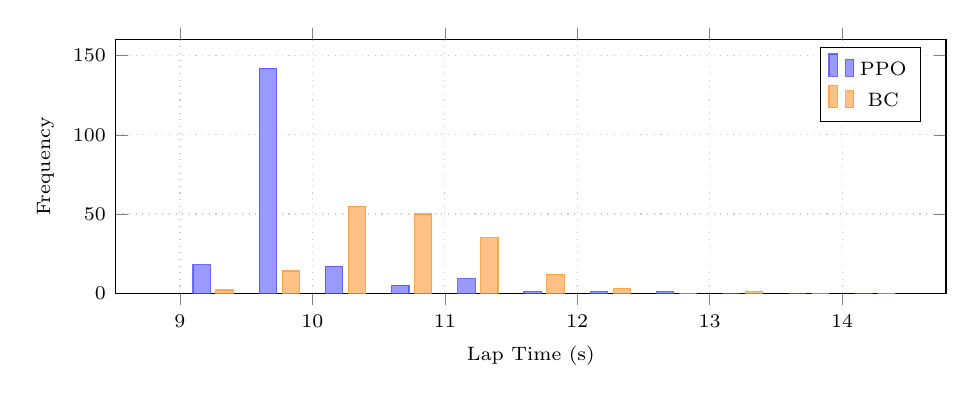
\begin{tikzpicture}
\begin{axis}[
    width=\columnwidth,
    height=4.8cm,
    xlabel={Lap Time (s)},
    ylabel={Frequency},
    xmin=8.8, xmax=14.5,
    ymin=0, ymax=160,
    bar width=0.22cm,
    legend pos=north east,
    legend style={font=\scriptsize},
    tick label style={font=\scriptsize},
    label style={font=\scriptsize},
    grid=major,
    grid style={dotted, gray!40},
    ybar,
    enlarge x limits=0.05,
]
\addplot[fill=blue!50, draw=blue!70, opacity=0.8]
coordinates {(9.25,18)(9.75,142)(10.25,17)(10.75,5)(11.25,9)(11.75,1)(12.25,1)(12.75,1)(13.25,0)(13.75,0)(14.25,0)};
\addplot[fill=orange!60, draw=orange!80, opacity=0.8]
coordinates {(9.25,2)(9.75,14)(10.25,55)(10.75,50)(11.25,35)(11.75,12)(12.25,3)(12.75,0)(13.25,1)(13.75,0)(14.25,0)};
\legend{PPO, BC}
\end{axis}
\end{tikzpicture}
\caption{Lap time frequency distribution for PPO and BC (successful episodes only,
         bin width = 0.5\,s). PPO bin 9.5--10.0\,s contains 142 episodes (71.7\%).
         PPO outliers $>$14.5\,s (4 episodes) are excluded for clarity.}
\label{fig:laptime_hist}
\end{figure}

The PPO distribution is sharply concentrated at the 9.5--10.0\,s bin (142 episodes, 71.7\% of completions). The BC distribution is broader and shifted rightward, centered around 10.0--11.5\,s, with no episodes below 9.25\,s. PPO outliers exceeding 14.5 seconds (4 episodes) are excluded from the histogram for visual clarity and reported separately in Table~\ref{tab:results_summary}. This confirms that while PPO achieves more frequent fast laps, BC exhibits a more symmetric distribution among its completions.

\subsubsection{Cumulative Reward per Episode (PPO)}

Fig.~\ref{fig:reward} shows the PPO cumulative reward per episode with a 10-episode rolling average.

\begin{figure}[!t]
\centering
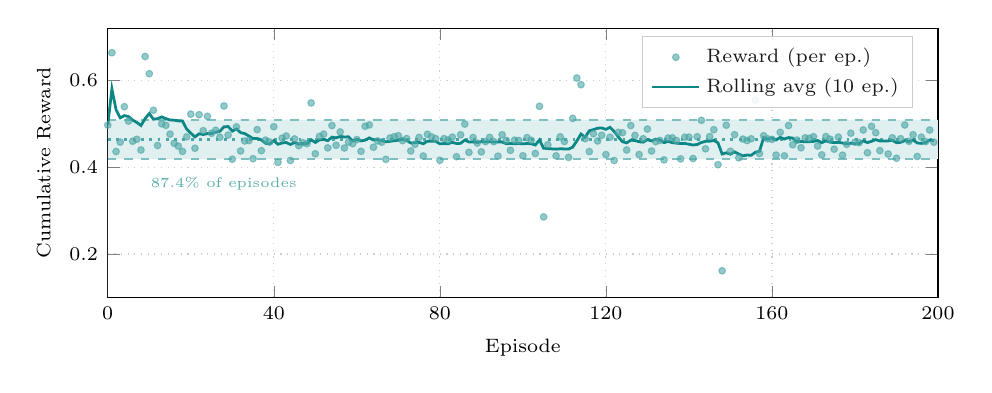
\begin{tikzpicture}
\begin{axis}[
    width=\columnwidth,
    height=5.0cm,
    xlabel={Episode},
    ylabel={Cumulative Reward},
    xmin=0, xmax=200,
    ymin=0.10, ymax=0.72,
    xtick={0,40,80,120,160,200},
    legend pos=north east,
    legend style={font=\scriptsize, cells={anchor=west},
                  fill=white, fill opacity=0.90, draw=gray!40},
    tick label style={font=\scriptsize},
    label style={font=\scriptsize},
    grid=major,
    grid style={dotted, gray!40},
    clip=true,
]

%% stable zone shading (mean ± 1 std: 0.419 – 0.509)
\addplot[draw=none, fill=teal!12, forget plot]
    coordinates {(0,0.419)(200,0.419)(200,0.509)(0,0.509)} \closedcycle;

%% stable zone boundary lines
\addplot[color=teal!50, line width=0.6pt, dashed, forget plot]
    coordinates {(0,0.419)(200,0.419)};
\addplot[color=teal!50, line width=0.6pt, dashed, forget plot]
    coordinates {(0,0.509)(200,0.509)};

%% mean line
\addplot[color=teal!70, line width=1.0pt, dotted, forget plot]
    coordinates {(0,0.464)(200,0.464)};

%% scatter
\addplot[only marks, mark=*, mark size=1.2pt,
         color=teal!70, opacity=0.60]
coordinates {(0,0.496948) (1,0.66363) (2,0.435967) (3,0.457701) (4,0.539232) (5,0.506107) (6,0.459668) (7,0.464249) (8,0.439558) (9,0.654892) (10,0.615321) (11,0.530893) (12,0.449833) (13,0.499688) (14,0.496304) (15,0.476018) (16,0.454817) (17,0.448351) (18,0.436241) (19,0.469866) (20,0.522147) (21,0.443538) (22,0.520861) (23,0.48405) (24,0.517017) (25,0.477994) (26,0.484944) (27,0.469027) (28,0.540965) (29,0.473978) (30,0.418281) (31,0.492787) (32,0.43727) (33,0.460256) (34,0.461169) (35,0.419498) (36,0.486531) (37,0.437906) (38,0.462261) (39,0.458009) (40,0.493199) (41,0.411164) (42,0.466765) (43,0.471723) (44,0.415362) (45,0.465112) (46,0.449568) (47,0.456179) (48,0.454056) (49,0.547899) (50,0.430784) (51,0.470873) (52,0.476074) (53,0.444455) (54,0.495805) (55,0.450304) (56,0.481146) (57,0.444067) (58,0.457506) (59,0.454175) (60,0.463583) (61,0.436504) (62,0.494148) (63,0.497231) (64,0.445859) (65,0.460335) (66,0.457474) (67,0.417939) (68,0.467166) (69,0.470101) (70,0.472453) (71,0.461181) (72,0.46593) (73,0.437361) (74,0.452565) (75,0.468554) (76,0.425733) (77,0.475717) (78,0.469821) (79,0.465736) (80,0.415864) (81,0.465725) (82,0.462637) (83,0.469149) (84,0.424154) (85,0.4745) (86,0.499209) (87,0.434109) (88,0.468248) (89,0.455379) (90,0.435183) (91,0.458779) (92,0.468645) (93,0.458728) (94,0.42529) (95,0.474616) (96,0.461395) (97,0.438642) (98,0.462233) (99,0.461489) (100,0.42618) (101,0.468044) (102,0.461765) (103,0.431568) (104,0.54019) (105,0.285474) (106,0.451806) (108,0.426094) (109,0.469928) (110,0.459068) (111,0.422457) (112,0.512375) (113,0.605191) (114,0.589932) (115,0.465669) (116,0.435869) (117,0.476944) (118,0.460301) (119,0.473568) (120,0.428965) (121,0.4689) (122,0.415302) (123,0.480166) (124,0.479251) (125,0.439551) (126,0.495802) (127,0.473155) (128,0.429066) (129,0.465529) (130,0.487734) (131,0.437184) (132,0.458647) (133,0.461566) (134,0.416832) (135,0.46707) (136,0.467573) (137,0.461439) (138,0.419068) (139,0.469009) (140,0.469195) (141,0.419924) (142,0.470164) (143,0.507847) (144,0.442251) (145,0.470576) (146,0.486297) (147,0.405792) (148,0.161234) (149,0.4965) (150,0.436597) (151,0.474847) (152,0.421528) (153,0.464665) (154,0.461289) (155,0.465326) (156,0.554122) (157,0.43143) (158,0.472336) (159,0.465254) (160,0.464037) (161,0.427805) (162,0.4802) (163,0.425965) (164,0.495807) (165,0.451649) (166,0.462547) (167,0.444756) (168,0.467649) (169,0.46649) (170,0.470179) (171,0.448669) (172,0.428344) (173,0.470532) (174,0.464475) (175,0.44139) (176,0.469292) (177,0.427528) (178,0.452531) (179,0.478198) (180,0.457522) (181,0.456417) (182,0.485632) (183,0.433286) (184,0.493972) (185,0.479371) (186,0.438114) (188,0.430185) (189,0.467653) (190,0.420534) (191,0.465538) (192,0.497152) (193,0.459454) (194,0.474756) (195,0.424607) (196,0.46916) (197,0.458765) (198,0.485533) (199,0.457419)};
\addlegendentry{Reward (per ep.)}

%% rolling avg
\addplot[color=teal!95, line width=1pt]
coordinates {(0,0.4969) (1,0.5803) (2,0.5322) (3,0.5136) (4,0.5187) (5,0.5166) (6,0.5085) (7,0.5029) (8,0.4959) (9,0.5118) (10,0.5236) (11,0.5104) (12,0.5117) (13,0.5159) (14,0.5117) (15,0.5086) (16,0.5082) (17,0.5066) (18,0.5062) (19,0.4877) (20,0.4784) (21,0.4697) (22,0.4768) (23,0.4752) (24,0.4773) (25,0.4775) (26,0.4805) (27,0.4826) (28,0.493) (29,0.4935) (30,0.4831) (31,0.488) (32,0.4796) (33,0.4773) (34,0.4717) (35,0.4658) (36,0.466) (37,0.4629) (38,0.455) (39,0.4534) (40,0.4609) (41,0.4527) (42,0.4557) (43,0.4568) (44,0.4522) (45,0.4568) (46,0.4531) (47,0.4549) (48,0.4541) (49,0.4631) (50,0.4569) (51,0.4628) (52,0.4638) (53,0.461) (54,0.4691) (55,0.4676) (56,0.4708) (57,0.4695) (58,0.4699) (59,0.4605) (60,0.4638) (61,0.4604) (62,0.4622) (63,0.4674) (64,0.4625) (65,0.4635) (66,0.4611) (67,0.4585) (68,0.4594) (69,0.461) (70,0.4619) (71,0.4644) (72,0.4616) (73,0.4556) (74,0.4563) (75,0.4571) (76,0.4539) (77,0.4597) (78,0.4599) (79,0.4595) (80,0.4538) (81,0.4543) (82,0.454) (83,0.4572) (84,0.4543) (85,0.4549) (86,0.4623) (87,0.4581) (88,0.4579) (89,0.4569) (90,0.4588) (91,0.4581) (92,0.4587) (93,0.4577) (94,0.4578) (95,0.4578) (96,0.454) (97,0.4545) (98,0.4539) (99,0.4545) (100,0.4536) (101,0.4545) (102,0.4538) (103,0.4511) (104,0.4626) (105,0.4437) (106,0.4427) (108,0.4415) (109,0.4423) (110,0.442) (111,0.4416) (112,0.4461) (113,0.4604) (114,0.4763) (115,0.4688) (116,0.4838) (117,0.4864) (118,0.4898) (119,0.4901) (120,0.4871) (121,0.4918) (122,0.4821) (123,0.4696) (124,0.4585) (125,0.4559) (126,0.4619) (127,0.4615) (128,0.4584) (129,0.4576) (130,0.4634) (131,0.4603) (132,0.4646) (133,0.4627) (134,0.4565) (135,0.4593) (136,0.4564) (137,0.4553) (138,0.4543) (139,0.4546) (140,0.4528) (141,0.451) (142,0.4522) (143,0.4568) (144,0.4594) (145,0.4597) (146,0.4616) (147,0.456) (148,0.4302) (149,0.433) (150,0.4297) (151,0.4352) (152,0.4303) (153,0.426) (154,0.4279) (155,0.4274) (156,0.4342) (157,0.4368) (158,0.4679) (159,0.4647) (160,0.4675) (161,0.4628) (162,0.4686) (163,0.4648) (164,0.4682) (165,0.4669) (166,0.4577) (167,0.459) (168,0.4586) (169,0.4587) (170,0.4593) (171,0.4614) (172,0.4562) (173,0.4607) (174,0.4575) (175,0.4565) (176,0.4572) (177,0.4555) (178,0.4539) (179,0.4551) (180,0.4538) (181,0.4546) (182,0.4604) (183,0.4566) (184,0.4596) (185,0.4634) (186,0.4603) (188,0.4605) (189,0.462) (190,0.4563) (191,0.4571) (192,0.4611) (193,0.4585) (194,0.4627) (195,0.4557) (196,0.4547) (197,0.4568) (198,0.4623) (199,0.4613)};
\addlegendentry{Rolling avg (10 ep.)}

%% annotations
\node[font=\tiny, color=teal!70, anchor=west]
    at (axis cs:202,0.509) {$+1\sigma$};
\node[font=\tiny, color=teal!70, anchor=west]
    at (axis cs:202,0.419) {$-1\sigma$};
\node[font=\tiny, color=teal!80, anchor=west]
    at (axis cs:202,0.464) {\textbf{$\mu$}};
\node[font=\tiny, fill=white, fill opacity=0.8,
      text=teal!80, align=center, anchor=north west]
    at (axis cs:8,0.4) {87.4\% of episodes};

\end{axis}
\end{tikzpicture}
\caption{PPO cumulative reward per inference episode with 10-episode rolling
         average. The shaded band marks mean\,$\pm$\,1\,std
         ($\mu=0.464$, $\sigma=0.045$), containing 87.4\% of episodes,
         indicating a stable converged policy.}
\label{fig:reward}
\end{figure}

The rolling average reward remains stable across the 200 episodes, fluctuating between approximately 0.44 and 0.52 with no systematic trend, confirming the PPO model had reached a stable performance regime prior to inference.

\subsubsection{Early-Episode Performance}

To assess initial inference behavior, the first 20 episodes of each agent were examined. The PPO agent completed all 20 laps with zero failures and a mean lap time of 10.21 seconds. The BC agent completed 15 out of 20 laps (75.0\% early completion rate) with 5 failures and a mean lap time of 10.74 seconds among successful laps. PPO's stability from episode zero is attributable to convergence achieved through 1,000 training iterations with eight parallel agents. BC's higher early failure rate reflects the covariate shift phenomenon, whereby states not represented in the ten-lap demonstration dataset cause compounding prediction errors \cite{ross2011reduction}.

\subsection{Statistical Comparison}

An independent-samples Welch's $t$-test was conducted on the lap times of successful episodes to assess whether the observed mean difference is statistically significant. The test yields $t = -7.66$, $df = 312.4$, confirming a statistically significant difference ($p \ll 0.001$) between the PPO mean ($\bar{x} = 9.99$\,s, $\sigma = 1.08$\,s, $n = 198$) and the BC mean ($\bar{x} = 10.68$\,s, $\sigma = 0.59$\,s, $n = 172$). The mean difference of 0.68 seconds is statistically robust, confirming that PPO's lap time advantage is not attributable to random variation.

\subsection{Comparative Discussion}

\subsubsection{Completion Reliability}

The most decisive difference between the two agents lies in lap completion reliability. PPO's 99.0\% completion rate versus BC's 86.0\% represents a gap of 13 percentage points, directly supporting the study's hypothesis that PPO achieves superior long-term reliability. BC's 28 failures are attributable to distributional shift: when the vehicle drifts into states rarely encountered in the expert demonstrations, the supervised regression policy offers no recovery mechanism. PPO, trained through reward-maximizing exploration, is exposed to a wider range of states. The track-deviation penalty $r_{track} = -10.0$ creates a corrective signal that encourages recovery behaviors, contributing to its superior completion rate.

\subsubsection{Lap Time and Consistency}

While PPO achieves a statistically significantly faster mean lap time, the comparison is nuanced. BC's lower standard deviation ($\sigma = 0.59$ vs.\ $\sigma = 1.08$) reflects more consistent lap execution across successful episodes. The imitation policy encodes a specific repeatable trajectory that minimizes within-distribution variance. PPO, optimizing for cumulative reward rather than trajectory replication, exhibits a wider performance envelope including both faster laps and occasional outlier episodes exceeding 15 seconds.

\subsubsection{Asymmetry in Training Conditions}

The two agents were trained under asymmetric conditions: PPO utilized eight parallel agents while BC used a single agent trained from ten expert demonstration laps. This asymmetry was a deliberate design choice to compensate for the inherent characteristics of each paradigm, and results should be interpreted accordingly.

\subsubsection{Summary}

In summary, the PPO agent outperforms BC on both completion rate and mean lap time under identical evaluation conditions. The Welch's $t$-test confirms the lap time advantage is statistically significant. BC demonstrates competitive consistency within successful episodes, indicating that imitation learning remains viable for stable, expert-like behavior within the demonstrated distribution. These findings are consistent with Chen et al.\ \cite{chen2024endtoend}, who argue that IL achieves competitive short-term performance while RL provides superior long-term adaptability.
\lipsum[11]

\section{Conclusions and Future Works}
\label{sec:conclusions}

\subsection{Conclusions}

This study presented a controlled empirical comparison between a Proximal Policy Optimization (PPO) agent and a Behavior Cloning (BC) agent for autonomous driving within Unreal Engine 5 using the Learning Agents plugin. Both agents were trained and evaluated on the same closed-loop racing track under identical inference conditions, with performance assessed over 200 episodes using lap completion rate, average lap time, and cumulative reward. The experimental results demonstrate that PPO achieves superior completion reliability, finishing 99.0\% of inference episodes (198/200) compared to 86.0\% for BC (172/200); the difference in failure count (3 vs.\ 28 episodes) indicates that reward-driven exploration enables PPO to learn recovery behaviors that BC---limited by its demonstration dataset---cannot replicate. Regarding lap times, PPO recorded a mean of $9.99 \pm 1.08$ seconds versus BC's $10.68 \pm 0.59$ seconds, a difference confirmed statistically significant by Welch's $t$-test ($t = -7.66$, $df = 312.4$, $p \ll 0.001$). While PPO achieves faster mean lap times, BC's lower standard deviation suggests that imitation learning produces more predictable behavior within the demonstrated state distribution. The higher failure rate of BC reflects the covariate shift problem: when the vehicle encounters states not represented in the ten-lap expert dataset, the policy lacks a recovery mechanism, resulting in episode termination---a limitation fundamental to pure Behavior Cloning \cite{ross2011reduction}. The results also confirm that the UE5 Learning Agents plugin is a viable platform for comparative machine learning research, providing an accessible, integrated environment supporting both PPO and BC without external simulators, extending the observation by Jorgensen \cite{jorgensen2023killers} to include the imitation learning component of the plugin.

\subsection{Future Works}

Several directions are identified for extending this research. Replacing pure Behavior Cloning with an online imitation learning algorithm such as DAgger \cite{ross2011reduction} could substantially mitigate covariate shift by iteratively collecting corrective expert feedback for states visited by the learned policy. Since the current evaluation was conducted exclusively on the training track, future work should assess the transfer performance of both agents on novel track configurations to quantify out-of-distribution generalization. Using BC to initialize the PPO policy before reinforcement learning fine-tuning could leverage the fast convergence of imitation learning with the long-term robustness of RL, as demonstrated in hierarchical planning settings \cite{bronstein2022hierarchical}. Collecting expert demonstrations from multiple drivers or across varied track conditions may also reduce BC's distributional sensitivity and improve completion rate without requiring reward engineering. Finally, incorporating richer sensory inputs---such as LiDAR-like raycasts or camera-based perception---could improve agent robustness and bring the simulation closer to real-world autonomous driving conditions.

\section{Open Data}
To support open science and reproducibility, the datasets, UE5 project configurations, and model checkpoints used in this project can be accessed through the following repository link: \url{https://github.com/placeholder-repo}

\section{Author Contributorship}
Aurelius Elbert: Conceptualization, Software, Investigation, Data Curation, Writing -- Original Draft, Writing -- Review \& Editing.
Davin Juandika: Conceptualization, Methodology, Writing -- Original Draft, Writing -- Review \& Editing.
Fransiskus Xaverius Kevin: Conceptualization, Formal Analysis, Visualization, Writing -- Original Draft, Writing -- Review \& Editing.
Gabriel Asael Tarigan: Supervision, Writing -- Review \& Editing.
Rhio Sutoyo: Supervision, Writing -- Review \& Editing.

% \section{Paper Organizational Structure}
% \label{sec:imrad}
% {\color{red}\textbf{Note: Please remove this tutorial section in the draft and final version of the paper.}}

% IMRAD (Introduction, Methods, Results, and Discussion) is a typical organizational structure (a document format) in scientific writing. 
% IMRaD is the most prominent norm for the structure of a scientific journal article of the original research type.
% The structure of IMRAD is shown in Fig. \ref{fig:imrad} and can be utilized to write a scientific paper. 
% Moreover, examples of academic papers that utilize IMRAD can be seen here: \cite{sutoyo2015dynamic, sutoyo2019designing, chowanda2021exploring}.

% \begin{figure}[htbp]
%     \centering
%     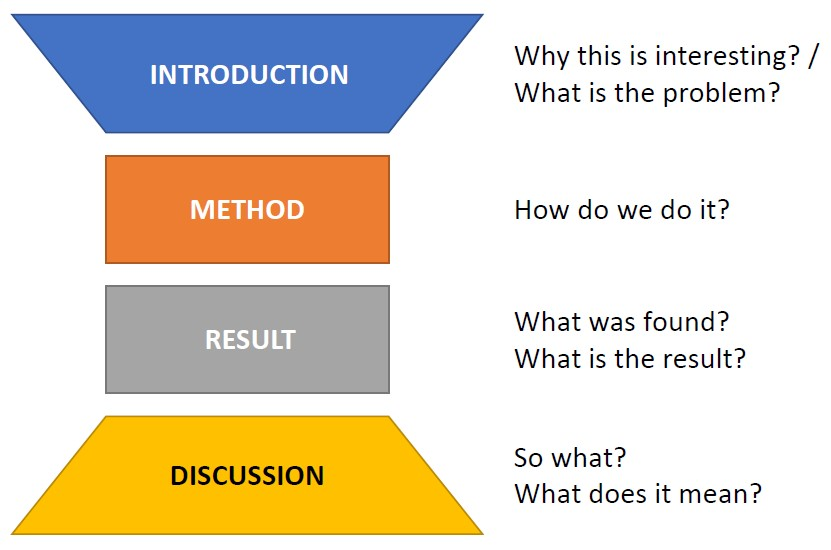
\includegraphics[width=0.45\textwidth]{images/IMRAD.jpg}
%     \caption{IMRAD}
%     \label{fig:imrad}
% \end{figure}

% \section{LaTeX Introduction}
% \label{sec:latex}
% {\color{red}\textbf{Note: Please remove this tutorial section in the draft and final version of the paper.}}

% LaTeX is a tool used to create professional-looking documents. 
% It is based on the WYSIWYM (what you see is what you mean) idea, meaning you only have to focus on the contents of your document, and the computer will take care of the formatting.
% For more information about \LaTeX, please visit this link\footnote{https://www.overleaf.com/learn/latex/Learn\_LaTeX\_in\_30\_minutes}.

% \section{Latex for Writing}
% {\color{red}\textbf{Note: Please remove this tutorial section in the draft and final version of the paper.}}

% This section of this template explains various features of latex for writing.

% \subsection{Captions, Labels, and References}
% After adding captions or labels, it is possible to mention them using cross-referencing features.
% For instance, the goal of this work has been discussed in Section \ref{sec:introduction}.

% \subsection{Adding Images}
% Examples for inserting figures. It uses the $graphicx$ package.
% The small image is shown in Fig. \ref{fig:small-image}, and the wide image is shown in Fig. \ref{fig:wide-image}.

% \begin{figure}[htbp]
%     \centering
%     
\includegraphics[width=0.2\textwidth]{images/small-image.jpg}
%     \caption{The caption of this image.}
%     \label{fig:small-image}
% \end{figure}

% \begin{figure*}[htbp]
%     \centering
%     
\includegraphics[width=0.95\textwidth]{images/wide-image.png}
%     \caption{The caption of this wide image.}
%     \label{fig:wide-image}
% \end{figure*}

% \subsection{Bold, Italics, and Underlining}
% Simple text formatting helps to highlight important concepts within a document and make it more readable. Using \textit{italics}, \textbf{bold}, or \underline{underlined} words can change the perception of the reader.

% \subsection{Add Citations}
% In the work of \cite{basar1995dynamic}, the problem of... \cite{achmad2021ant} and \cite{sutoyo2019designing}.
% For more results on this topic, we refer readers to \cite{dirac, einstein} and the references therein...

% \subsection{Using Lists}
% The itemized environment for bulleted (unordered) lists.
% \begin{itemize}
%   \item List entries start with the \verb|\item| command.
%   \item Individual entries are indicated with a black dot, a so-called bullet.
%   \item The text in the entries may be of any length.
% \end{itemize}

% Numbered (ordered) lists have the same syntax but use the enumerate environment.
% \begin{enumerate}
%   \item Items are numbered automatically.
%   \item The numbers start at 1 with each use of the \texttt{enumerate} environment.
%   \item Another entry in the list
% \end{enumerate}

% \subsection{Create Tables}
% Tables are important for showing data. Use this website\footnote{https://www.tablesgenerator.com/latex\_tables} to create tables. 
% The Table \ref{tab:example-table} shows a simple table. An example of a wide table that shows the best-selling individual books is shown in Table \ref{tab:best-selling-books}.

% \begin{table}[htbp]
%     \caption{Table Type Styles}
%     \begin{center}
%     \begin{tabular}{|c|c|c|c|}
%     \hline
%     \textbf{Table}&\multicolumn{3}{|c|}{\textbf{Table Column Head}} \\
%     \cline{2-4} 
%     \textbf{Head} & \textbf{\textit{Table column subhead}}& \textbf{\textit{Subhead}}& \textbf{\textit{Subhead}} \\
%     \hline
%     copy& More table copy$^{\mathrm{a}}$& &  \\
%     \hline
%     \multicolumn{4}{l}{$^{\mathrm{a}}$Sample of a Table footnote.}
%     \end{tabular}
%     \label{tab:example-table}
%     \end{center}
% \end{table}

% \begin{table*}[htbp]
% \centering
% \caption{List of best-selling individual books}
% \label{tab:best-selling-books}
% \resizebox{\textwidth}{!}{%
% \begin{tabular}{lllrrl}
% \hline
% \textbf{Book} & \textbf{Author(s)} & \textbf{Original   language} & \textbf{First published} & \textbf{Approximate   sales} & \textbf{Genre} \\ \hline
% A Tale of Two   Cities                     & Charles Dickens          & English & 1859 & 200,000,000 & Historical fiction \\
% The Little   Prince                        & Antoine de Saint-Exupéry & French  & 1943 & 200,000,000 & Novella            \\
% Harry Potter   and the Philosopher's Stone & J. K. Rowling            & English & 1997 & 120,000,000 & Fantasy            \\
% And Then There   Were None                 & Agatha Christie          & English & 1939 & 100,000,000 & Mystery            \\
% Dream of the   Red Chamber                 & Cao Xueqin               & Chinese & 1791 & 100,000,000 & Family saga        \\
% The Hobbit                                 & J. R. R. Tolkien         & English & 1937 & 100,000,000 & Fantasy            \\ \hline
% \end{tabular}%
% }
% \end{table*}

% \subsection{Equations}
% Examples for writing equations. The equation of the Law of Gravity is shown in (\ref{eq:law-of-gravity}).
% Use this website\footnote{https://latex.codecogs.com/eqneditor/editor.php} to create a more complex equation.

% \begin{equation}
% \label{eq:law-of-gravity}
% F = G\frac{m_1m_2}{r^2}
% \end{equation}

% Be sure that the symbols in your equation have been defined before or immediately following 
% the equation. Use ``\eqref{eq:law-of-gravity}'', not ``Eq.~\eqref{eq:law-of-gravity}'' or ``equation \eqref{eq:law-of-gravity}'', except at 
% the beginning of a sentence: ``Equation \eqref{eq:law-of-gravity} is . . .''

% \subsection{Algorithms}
% Examples for inserting algorithms. It uses $algorithm$ and $algpseudocode$ packages. The algorithm is shown in Algorithm \ref{alg:cap}.

% \begin{algorithm}
%     \caption{An algorithm with caption}
%     \label{alg:cap}
%     \begin{algorithmic}[1]
%     \Require $n \geq 0$
%     \Ensure $y = x^n$
%     \State $y \gets 1$
%     \State $X \gets x$
%     \State $N \gets n$
%     \While{$N \neq 0$}
%     \If{$N$ is even}
%         \State $X \gets X \times X$
%         \State $N \gets \frac{N}{2}$  \Comment{This is a comment}
%     \ElsIf{$N$ is odd}
%         \State $y \gets y \times X$
%         \State $N \gets N - 1$
%     \EndIf
%     \EndWhile
%     \end{algorithmic}
% \end{algorithm}

% \section{Some Common Mistakes}
% \label{SCM}
% {\color{red}\textbf{Note: Please remove this tutorial section in the draft and final version of the paper.}}

% Please avoid these common mistakes in the writing. 
% Using software such as Grammarly\footnote{https://www.grammarly.com/} as a writing assistant is recommended.
% \begin{itemize}
% \item Using we in academic writing is generally not recommended because it can introduce ambiguity and subjectivity. Please use passive voice, third-person perspective, and noun phrases (e.g., "This study proposes a new framework for text classification."). 
% \item The abbreviation ``i.e.'' means ``that is'', and the abbreviation ``e.g.'' means ``for example''.
% \item The word ``data'' is plural, not singular.
% \item In your paper title, if the words ``that uses'' can accurately replace the word ``using'', capitalize the ``u''; if not, keep using lower-cased.
% \item Be aware of the different meanings of the homophones ``affect'' and ``effect'', ``complement'' and ``compliment'', ``discreet'' and ``discrete'', ``principal'' and ``principle''.
% \end{itemize}

\bibliographystyle{IEEEtran}
\bibliography{bibliography}

\end{document}